% !TeX root = ../thuthesis-example.tex

\chapter{机器学习平台体系架构}
\label{chap:architecture}

与数据库、中间件等系统软件不同,机器学习平台的性质更偏向于信息化业务应用系统。
这样会造成的一种假象是,任何开发人员都可以轻易地上手开发构建机器学习平台。
在当今普遍追求开发短平快的不良风气下,很容易因忽略设计和规划而导致构建成型的机器学习平不可维护、不可扩展、不可靠等问题。
因此,本节作为机器学习平台研究的第一部分内容,着重围绕机器学习平台的体系架构设计展开讨论,以期为机器学习平台的设计和实现提供一些参考。


\section{总体架构}
\label{sec:architecture-overview}

图\ref{fig:architecture-overview}展示了云原生机器学习平台的总体架构。
从整体的角度上看,云原生背景下的机器学习平台向下依托云基础设施,得到CPU、GPU、存储等硬件资源和数据库、中间件、监控基础系统软件的支持,并充分发挥云计算的弹性和扩展性实现自身的高吞吐、高可用等特性;
向上,机器学习平台输出机器学习研发的相关能力,支撑机器学习应用的开发和落地。

\begin{figure}
  \centering
  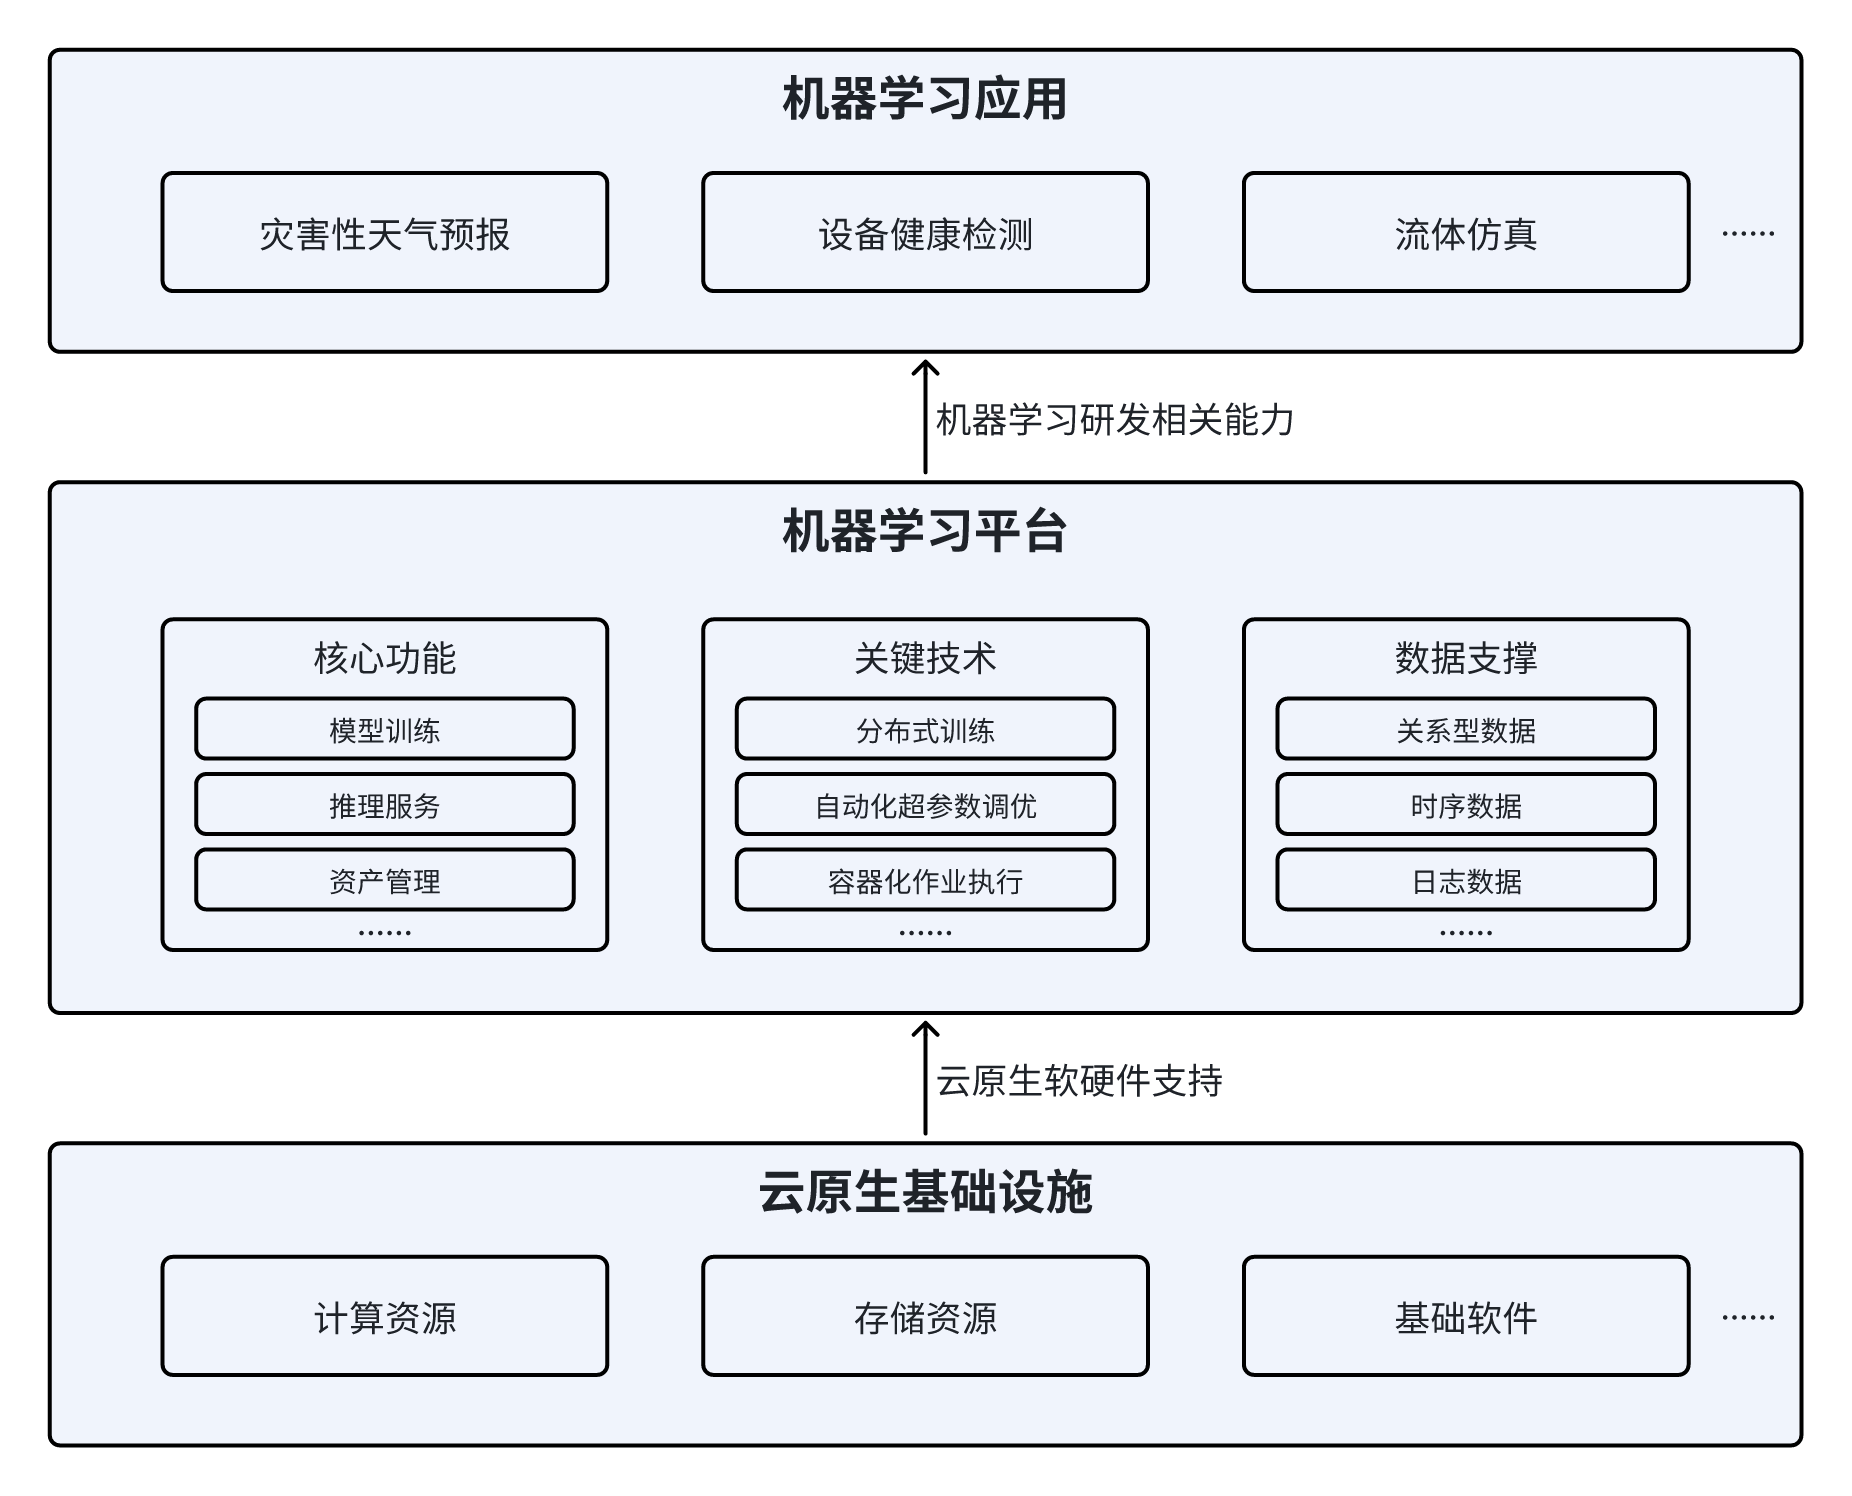
\includegraphics[width=0.98\linewidth]{architecture-overview.png}
  \caption{机器学习平台总体架构}
  \label{fig:architecture-overview}
\end{figure}

从外部视角看,任何软件系统的能力边界是决定其内部架构的关键性指导思想,机器学习平台也不例外,需要首先定义其能力体系。
聚焦到机器学习平台内部的视角,功能体系、技术体系和数据体系是其架构的重要组成部分:从能力体系出发,由核心功能支撑能力的输出,并通过技术体系和数据体系支撑功能的具体实现。
最后,交互体系是机器学习平台与用户之间的接口,是机器学习平台的外部表现形式,也决定着平台的组织运用方式。
因此,本章的后续内容将围绕能力体系、功能体系、技术体系、数据体系和交互体系几个方面展开讨论。


\section{能力体系}

基于\ref{sec:architecture-overview}节所述的总体架构,机器学习平台对外输出的主要是机器学习研发相关的能力,主要包括机器学习模型生成的相关作业能力和研发管理的相关能力,如图\ref{fig:architecture-capabilities}所示。

\begin{figure}
  \centering
  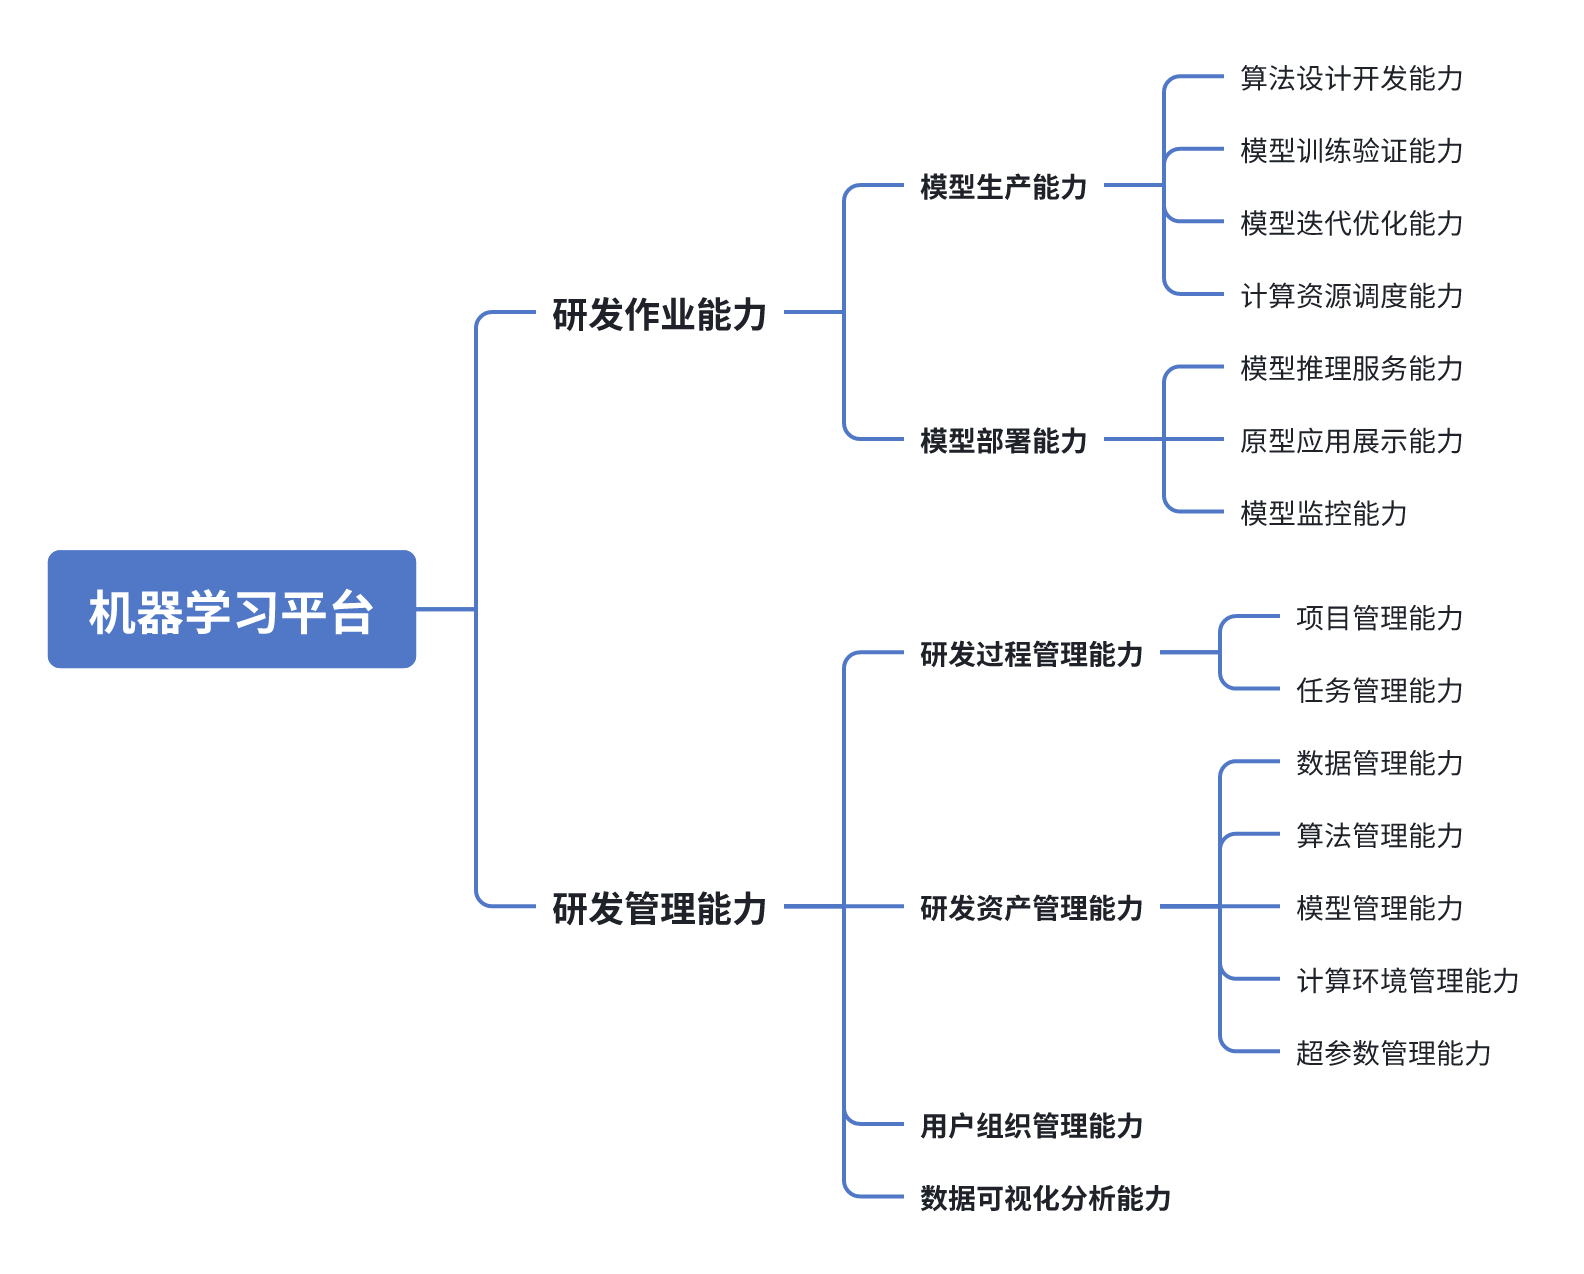
\includegraphics[width=0.98\linewidth]{architecture-capabilities.png}
  \caption{机器学习平台能力体系}
  \label{fig:architecture-capabilities}
\end{figure}

模型研发作业能力主要分为生产和部署两部分。
模型生产能力是面向模型开发训练的能力,最终输出训练好的模型,覆盖算法设计开发、模型训练验证、模型迭代优化以及训练验证所必需的计算资源调度。
模型部署能力是面向模型服务部署的能力,最终输出可供业务应用调用的推理服务,覆盖模型导出、模型推理服务封装以及模型监控。

研发管理能力主要分为过程管理、资产管理、用户管理和数据可视化分析四部分。
过程管理能力以项目管理为中心,对机器学习作业任务进行管理,可结合用户组织对任务分工进行管理,可支撑机器学习研发的所有作业流程。
资产管理能力围绕数据、算法、模型、超参数、计算环境等机器学习研发所需的各类资产进行管理,支撑资产的追溯和实验任务的复现。
用户组织管理能力是实现上述管理能力的基础,支撑用户组织的管理、权限控制、资源分配等功能。
数据可视化分析能力是面向管理者提供系统的统计数据分析与可视化能力,辅助管理决策。


\section{功能体系}

依照能力体系的划分方式,机器学习平台的功能主要分为研发作业子系统和研发管理子系统两部分,如图\ref{fig:architecture-features}所示。

\begin{figure}
  \centering
  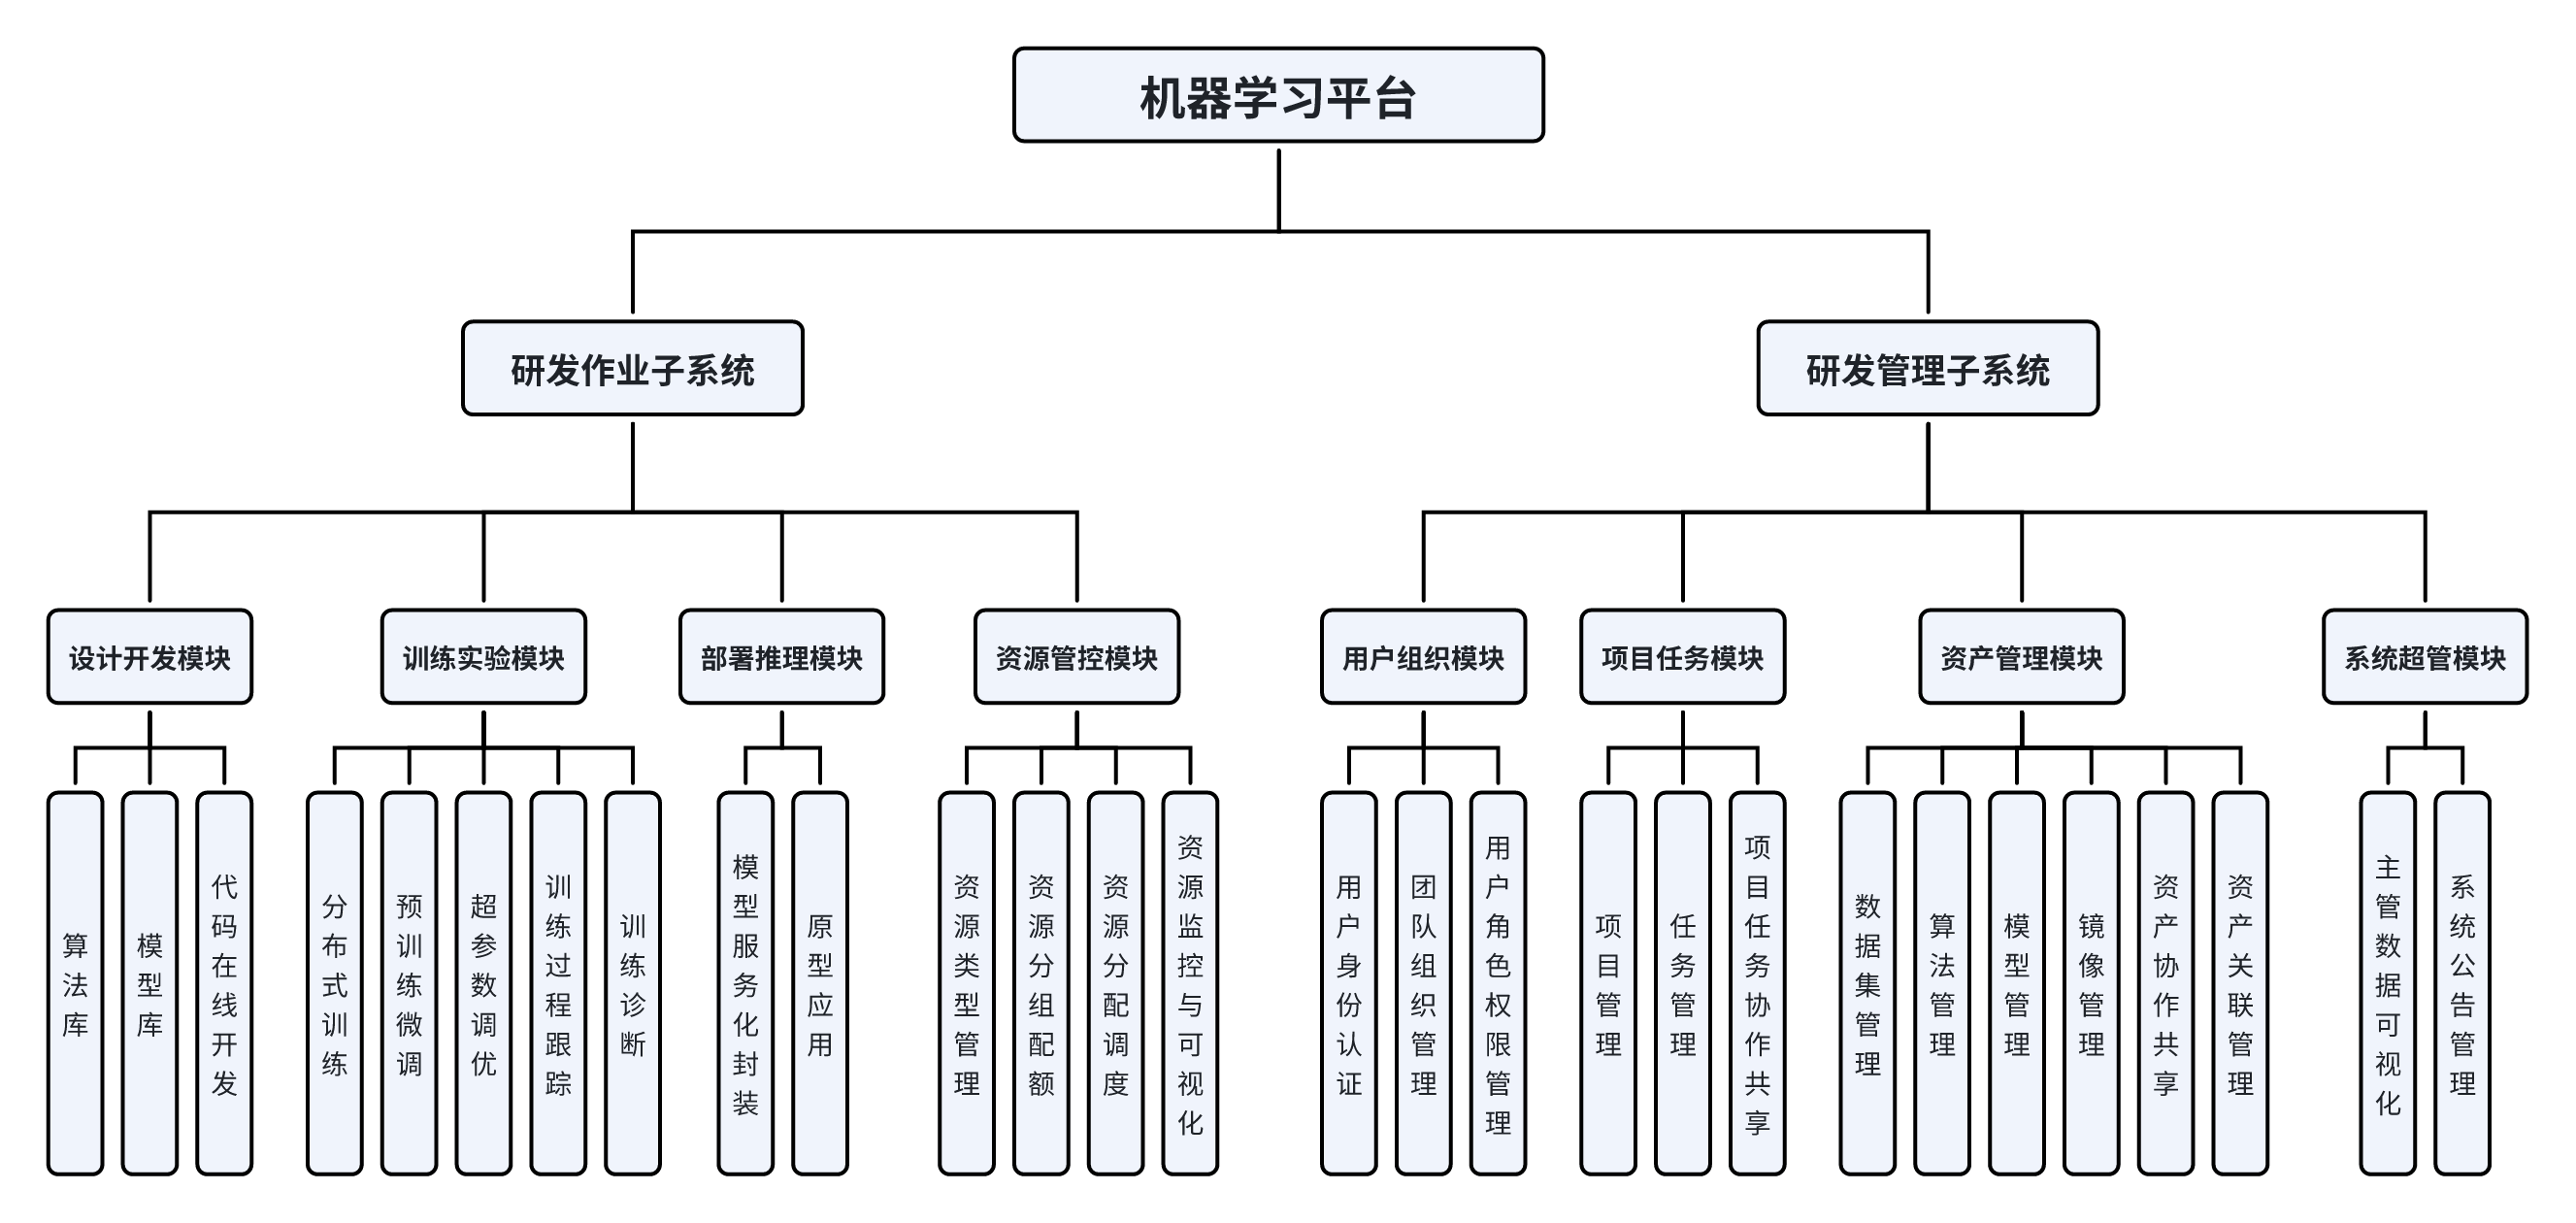
\includegraphics[width=0.98\linewidth]{architecture-features.png}
  \caption{机器学习平台功能体系}
  \label{fig:architecture-features}
\end{figure}

研发作业子系统包括设计开发模块、训练实验模块、部署推理模块以及资源管控模块。
设计开发模块提供算法库、模型库和代码在线开发功能,支持用户灵活调用算法和模型资源,并提供实时开发和调试环境。
训练实验模块则支持分布式训练和预训练微调,同时提供超参数优化工具、训练过程监控功能,以及对训练中潜在问题进行诊断的能力。
部署推理模块专注于将模型服务化,通过封装的API实现模型在线调用,同时支持原型应用快速上线以验证效果。
资源管控模块负责管理和分类计算与存储资源,并对资源进行分组、分配,支持资源使用的实时可视化和监控。

研发管理子系统主要负责用户、任务、项目以及平台资产的管理。
用户组织模块提供用户身份认证、团队管理和角色权限控制,以保障用户的操作安全并规范权限分配。
项目任务模块支持项目的创建和任务分解,实现任务分配与团队协作,并提供共享机制以提升整体效率。
资产管理模块涵盖数据集、算法、模型和容器镜像的存储和管理,支持资产间的关联关系建立,进一步提高平台资源的可追溯性和复用能力。
系统超管模块为平台管理员提供管理入口,支持系统公告的发布以及关键数据的可视化展示,用于全面掌控平台运行状态。


\section{数据体系}

图\ref{fig:architecture-data}展示了机器学习平台的数据体系,涵盖关系型数据、时序数据、非结构化数据和日志数据四个主要类别。

\begin{figure}
  \centering
  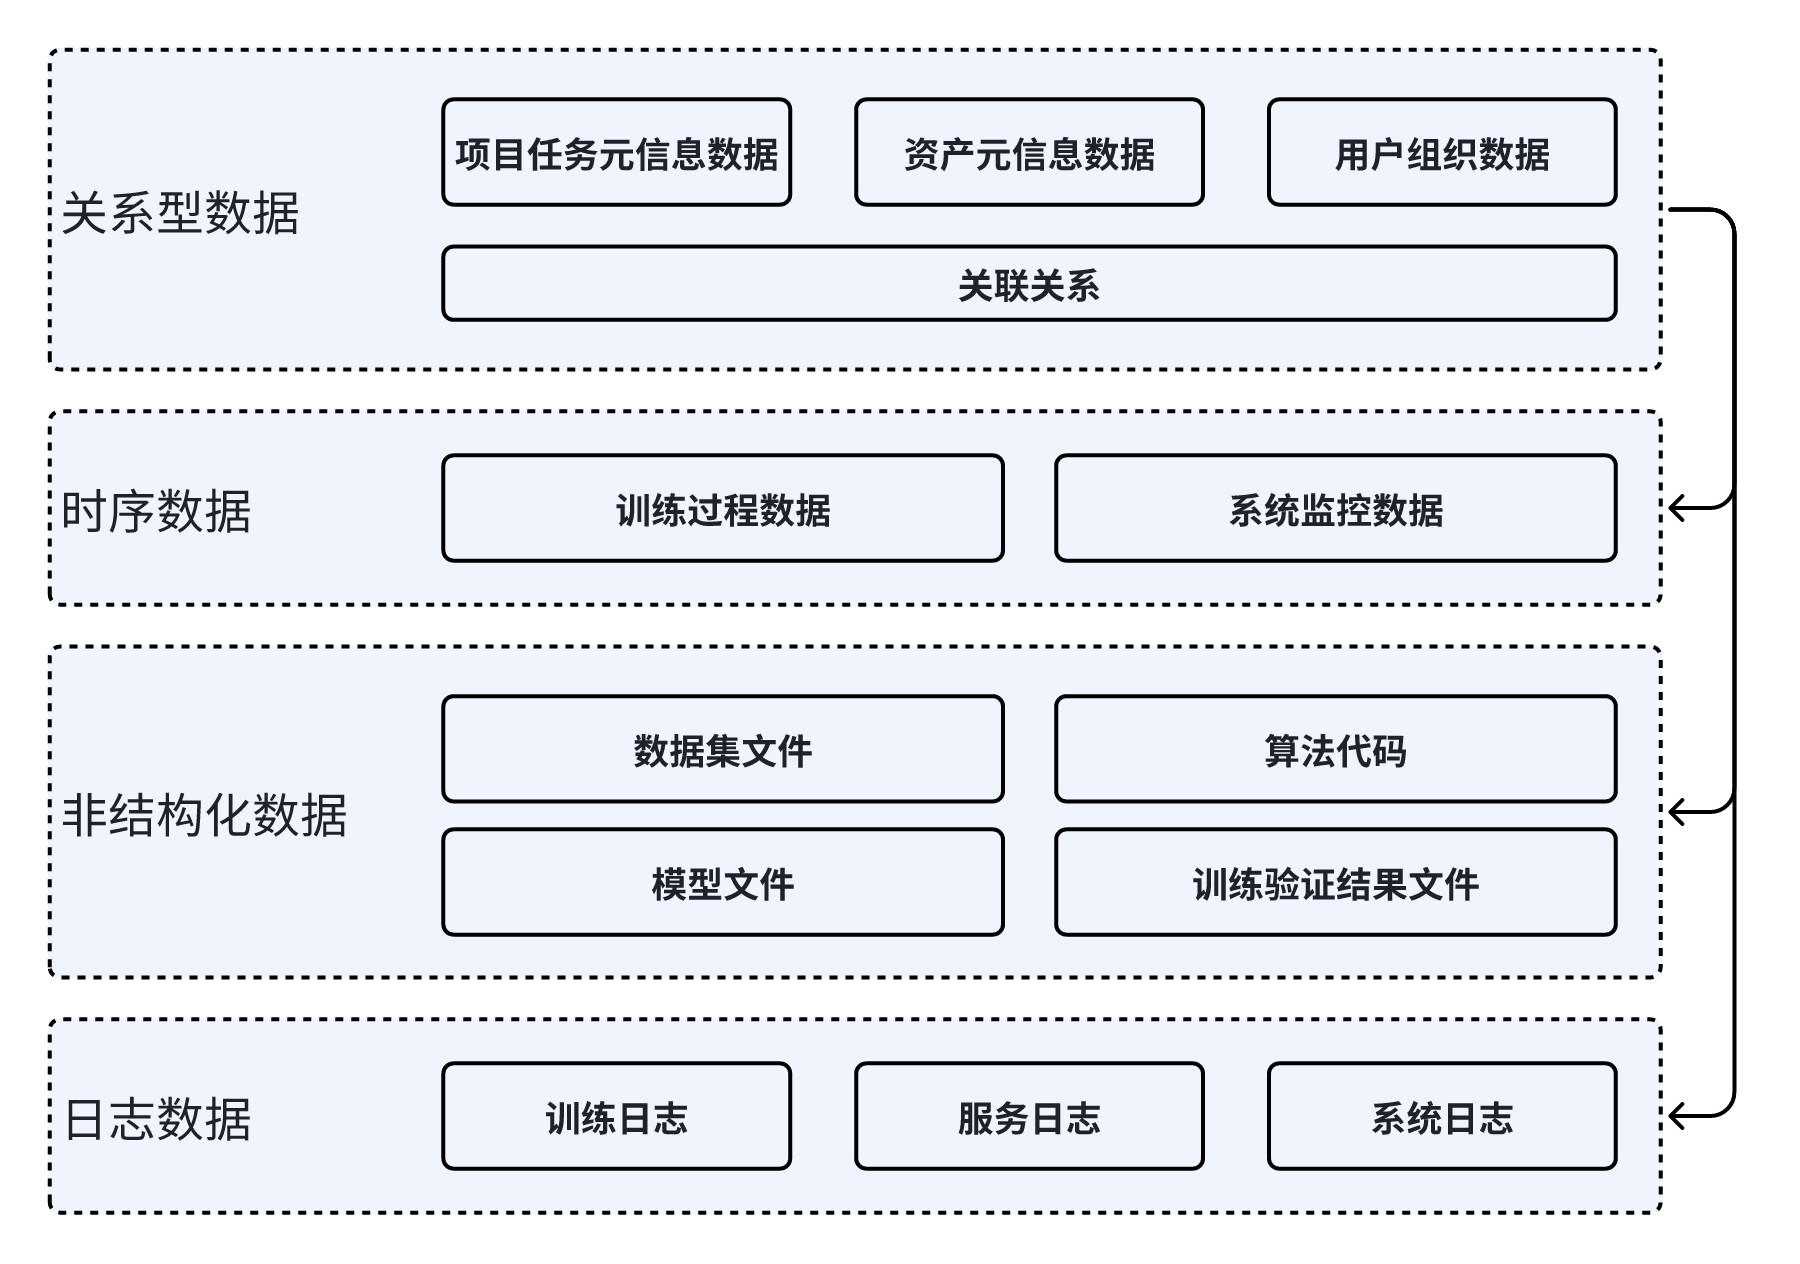
\includegraphics[width=0.8\linewidth]{architecture-data.png}
  \caption{机器学习平台数据体系}
  \label{fig:architecture-data}
\end{figure}

关系型数据包括项目任务元信息数据、资产元信息数据和用户组织数据,这些数据通过建立关联关系来实现信息的有序管理与查询,支撑系统的基本结构化操作。时序数据主要包括训练过程数据和系统监控数据,用于记录训练运行的时间变化信息和系统资源的动态状态,为实时分析与性能优化提供支撑。非结构化数据涵盖数据集文件、算法代码、模型文件和训练验证结果文件,存储形式多样,用于模型开发和实验过程中的各种需求。日志数据包括训练日志、服务日志和系统日志,用于记录系统运行、模型推理服务和训练任务的操作历史,为故障排查和性能评估提供可靠依据。数据体系的各部分通过交互和反馈机制共同作用,构成平台的数据支撑框架。


\section{技术体系}

图\ref{fig:architecture-technologies}描述了云原生机器学习平台的技术体系,底层依托云原生领域的事实标准Kubernetes,向上构建基础环境和平台。

\begin{figure}
  \centering
  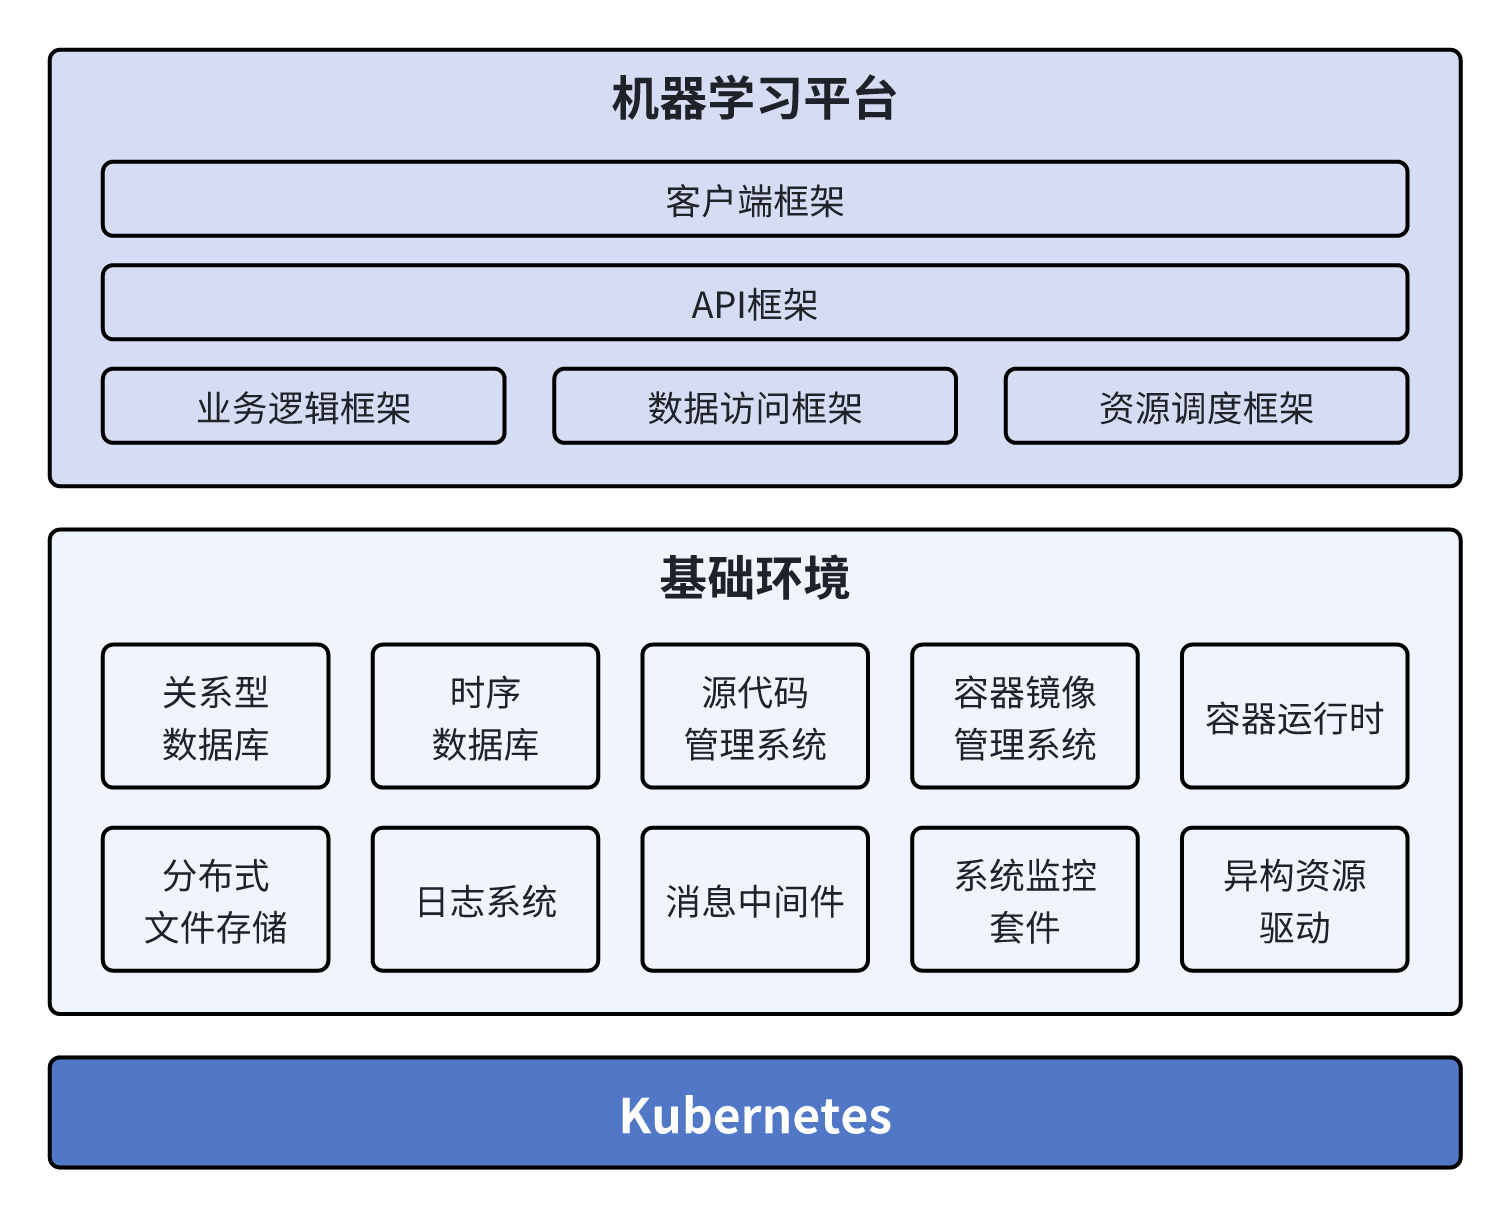
\includegraphics[width=0.8\linewidth]{architecture-technologies.png}
  \caption{机器学习平台技术体系}
  \label{fig:architecture-technologies}
\end{figure}

机器学习平台层由客户端框架、API框架、业务逻辑框架、数据访问框架和资源调度框架组成。客户端框架用于提供用户交互界面,API框架负责对外暴露统一的编程接口,业务逻辑框架实现具体的业务处理逻辑,数据访问框架用于高效读取和写入平台的数据,资源调度框架实现资源的动态分配与优化。

基础环境层包括支持平台运行的关键服务和工具,如关系型数据库、时序数据库、源码管理系统、容器镜像管理系统和容器运行时,用于存储结构化数据、时间序列数据和代码资源,同时为模型训练、部署等任务提供镜像管理和运行支持。分布式文件存储提供大规模数据存储能力,日志系统记录平台运行的行为日志,消息中间件负责异步任务通信,系统监控套件实现平台运行状态的实时监测,异构资源驱动支持GPU、NPU等不同硬件资源的接入和管理。


\section{交互体系}

图\ref{fig:architecture-interfaces}展示了机器学习平台的交互体系,包括Web页面、SDK和CLI三种主要的客户端形式,以满足不同场景下的用户需求。

\begin{figure}
  \centering
  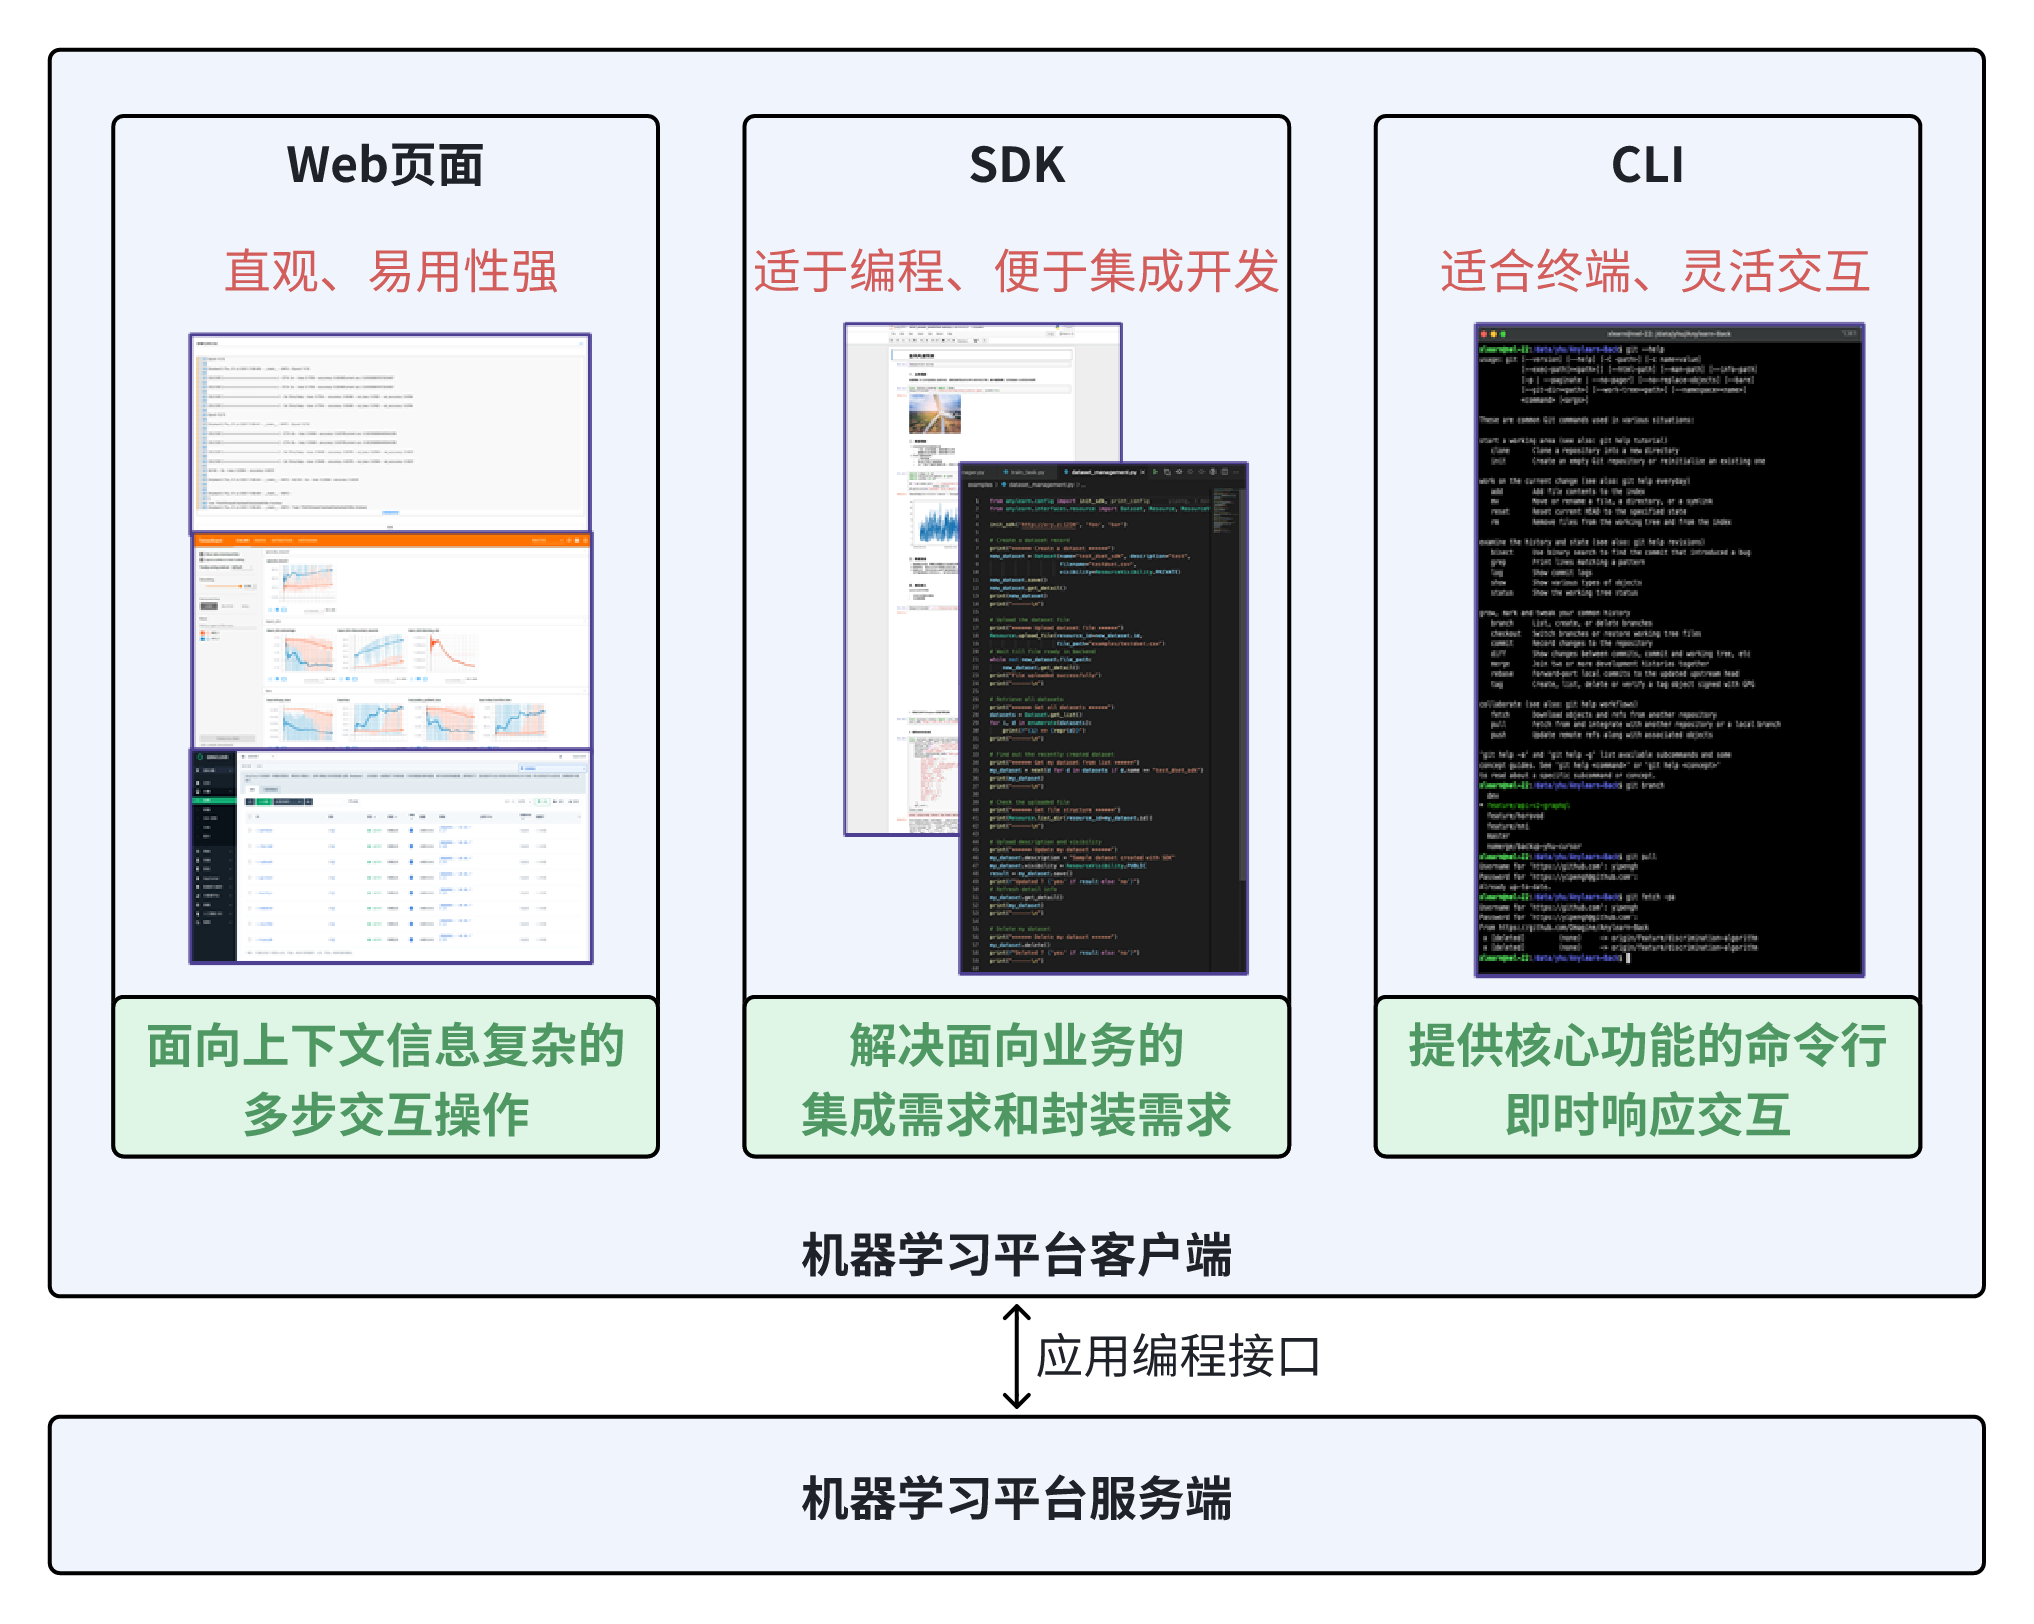
\includegraphics[width=0.98\linewidth]{architecture-interfaces.png}
  \caption{机器学习平台交互体系}
  \label{fig:architecture-interfaces}
\end{figure}

Web页面注重直观性和易用性,适用于需要上下文信息复杂、多步骤交互操作的场景。
通过可视化界面,用户可以直观地查看数据和模型状态,执行操作步骤,适合对系统功能进行全面了解和管理。
SDK面向业务集成需求,提供编程接口,便于开发者在自己的工作流或系统中直接调用平台功能,实现高度定制化和自动化的操作。
CLI提供简洁高效的命令行界面,适用于终端环境中的灵活交互,专注于核心功能的即时调用,适合高级用户和开发者快速完成特定任务。
三个交互层通过应用编程接口与平台服务端连接,形成功能完备且灵活的用户交互体系。
